\documentclass{book}

\usepackage{graphicx,amscd,amsmath,amssymb,verbatim}
%\usepackage[dvips]{hyperref}	% for hyperlinks
\usepackage{url}
\usepackage{epstopdf} % so can use EPS or PDF figures
\usepackage{appendix}	% for finer control of the appendix

\DeclareMathSymbol{\Gamma}{\mathalpha}{letters}{"00}	% Greek capital letters in italics
\DeclareMathSymbol{\Delta}{\mathalpha}{letters}{"01}
\DeclareMathSymbol{\Theta}{\mathalpha}{letters}{"02}
\DeclareMathSymbol{\Lambda}{\mathalpha}{letters}{"03}
\DeclareMathSymbol{\Xi}{\mathalpha}{letters}{"04}
\DeclareMathSymbol{\Pi}{\mathalpha}{letters}{"05}
\DeclareMathSymbol{\Sigma}{\mathalpha}{letters}{"06}
\DeclareMathSymbol{\Upsilon}{\mathalpha}{letters}{"07}
\DeclareMathSymbol{\Phi}{\mathalpha}{letters}{"08}
\DeclareMathSymbol{\Psi}{\mathalpha}{letters}{"09}
\DeclareMathSymbol{\Omega}{\mathalpha}{letters}{"0A}

%%%%%%%%%%%%%%%%%%%%%%%%%%%%%%%%%%%%%%%%
%%%%%%%%%%%%%%%%%%%%%%%%%%%%%%%%%%%%%%%%
\begin{document}

\frontmatter

\begin{titlepage}
	\begin{center}

		\huge{This is the Title}

		\vspace{2.5cm}

		\LARGE{Jane Q. Doe}\\ 
		\LARGE{Physics Department}\\
		\LARGE{The College of Wooster}\\
		
		\vspace{0.5cm}
		
		\large A dissertation submitted in partial fulfillment 
		of the requirements of  Senior Independent Study in Physics at The College of Wooster\\
		
		\vspace{2.5cm}
		
		\begin{table}[h!]
			\begin{center}
				\begin{tabular}{c}
				
					\large{\emph{Adviser}}\\
					\large{Dr. John F. Lindner}\\
					\vspace{0.5cm}\\
					\hline
					
					\vspace{1.0cm}\\
					\large{\emph{Second Reader}}\\
					\large{Dr. Del B. Chord}\\
					\vspace{0.5cm}\\
					\hline
					
				\end{tabular}
			\end{center}
		\end{table}
		
		\vspace{2.5cm}

		\large{\today}

	\end{center}
\end{titlepage}

%%%%%%%%%%%%%%%%%%%%%%%%%%%%%%%%%%%%%%%%
\chapter*{Abstract}\addcontentsline{toc}{chapter}{Abstract}

This is dummy text. This is dummy text. This is dummy text. This is dummy text. This is dummy text. This is dummy text. This is dummy text. This is dummy text. This is dummy text. This is dummy text. This is dummy text. This is dummy text. This is dummy text. This is dummy text. This is dummy text. This is dummy text. This is dummy text. This is dummy text. This is dummy text. This is dummy text. This is dummy text. This is dummy text. This is dummy text. This is dummy text. This is dummy text. This is dummy text. 

This is dummy text. This is dummy text. This is dummy text. This is dummy text. This is dummy text. This is dummy text. This is dummy text. This is dummy text. This is dummy text. This is dummy text. This is dummy text. This is dummy text. This is dummy text. This is dummy text. This is dummy text. This is dummy text. This is dummy text. This is dummy text. This is dummy text. This is dummy text. This is dummy text. This is dummy text. This is dummy text. This is dummy text. This is dummy text. This is dummy text. elegant text. This elegant text. This elegant text. This elegant text. This elegant text. 

%%%%%%%%%%%%%%%%%%%%%%%%%%%%%%%%%%%%%%%%
\chapter*{Acknowledgments}\addcontentsline{toc}{chapter}{Acknowledgments}

This is dummy text. This is dummy text. This is dummy text. This is dummy text. This is dummy text. This is dummy text. This is dummy text. This is dummy text. This is dummy text. This is dummy text. This is dummy text. This is dummy text. This is dummy text. This is dummy text. This is dummy text. This is dummy text. This is dummy text. This is dummy text. This is dummy text. This is dummy text. This is dummy text. This is dummy text. This is dummy text. This is dummy text. This is dummy text. This is dummy text. 

This is dummy text. This is dummy text. This is dummy text. This is dummy text. This is dummy text. This is dummy text. This is dummy text. This is dummy text. This is dummy text. This is dummy text. This is dummy text. This is dummy text. This is dummy text. This is dummy text. This is dummy text. This is dummy text. This is dummy text. This is dummy text. This is dummy text. This is dummy text. This is dummy text. This is dummy text. This is dummy text. This is dummy text. This is dummy text. This is dummy text. 

%%%%%%%%%%%%%%%%%%%%%%%%%%%%%%%%%%%%%%%%
%%%%%%%%%%%%%%%%%%%%%%%%%%%%%%%%%%%%%%%%
\tableofcontents
\setcounter{tocdepth}{2}
\listoftables
\listoffigures

%%%%%%%%%%%%%%%%%%%%%%%%%%%%%%%%%%%%%%%%
%%%%%%%%%%%%%%%%%%%%%%%%%%%%%%%%%%%%%%%%
%%%%%%%%%%%%%%%%%%%%%%%%%%%%%%%%%%%%%%%%
\mainmatter

%%%%%%%%%%%%%%%%%%%%%%%%%%%%%%%%%%%%%%%%
%%%%%%%%%%%%%%%%%%%%%%%%%%%%%%%%%%%%%%%%
\chapter{Introduction}\label{introduction}

\section{Basics}

This is text. This is \textbf{bold} text. This is text with \emph{emphasis}. This is ``double quotes". 

Paragraphs are separated by one or more blank lines. 

% %%%%%%%%%%%%%%%%%%%%%%%%%%%%%%
\section{Math \& Citations}	% "&" is a special character
Examples of inline math are $\alpha = \sqrt{\gamma^2 + \Gamma^2}$ and $\vec{v} = 7 \hat{x} - 5 \hat{y}$ and $\vec u \times \vec v$ and $c = (2.99 \pm 0.01) \times 10^8$ m/s. One example of block (display) math is
%
\begin{equation}
	\int_0^1x^2 dx = \frac{1}{3},
	\label{myIntegral}
\end{equation}
%
and a second example is
%
\begin{equation}
	\xi = \alpha \left( \frac{1}{ \omega_0^2 + \omega^2 } \right).
	\label{signal}
\end{equation}
%
Note how block math is punctuated like words in a sentence! The block math equations are automatically numbered. We can reference Eq. \ref{myIntegral} or Eq. \ref{signal} by inserting labels in the block, but then we must compile \LaTeX\ twice.

We can readily cite articles \cite{Chenciner2000}  and books \cite{Gleick1987} and URLs \cite{Lindner2015} in our bibliography, but now we must compile \LaTeX, Bib\TeX,  \LaTeX, \LaTeX.

% %%%%%%%%%%%%%%%%%%%%%%%%%%%%%%
\section{Figures \& Tables}
We can also include figures, but first we need to use package ``graphicx" under document class. We can reference Fig. \ref{SchematicDiagram} like equations. All figures should have captions.

\begin{figure}[ht] % "ht" = here or top
	\begin{center}
		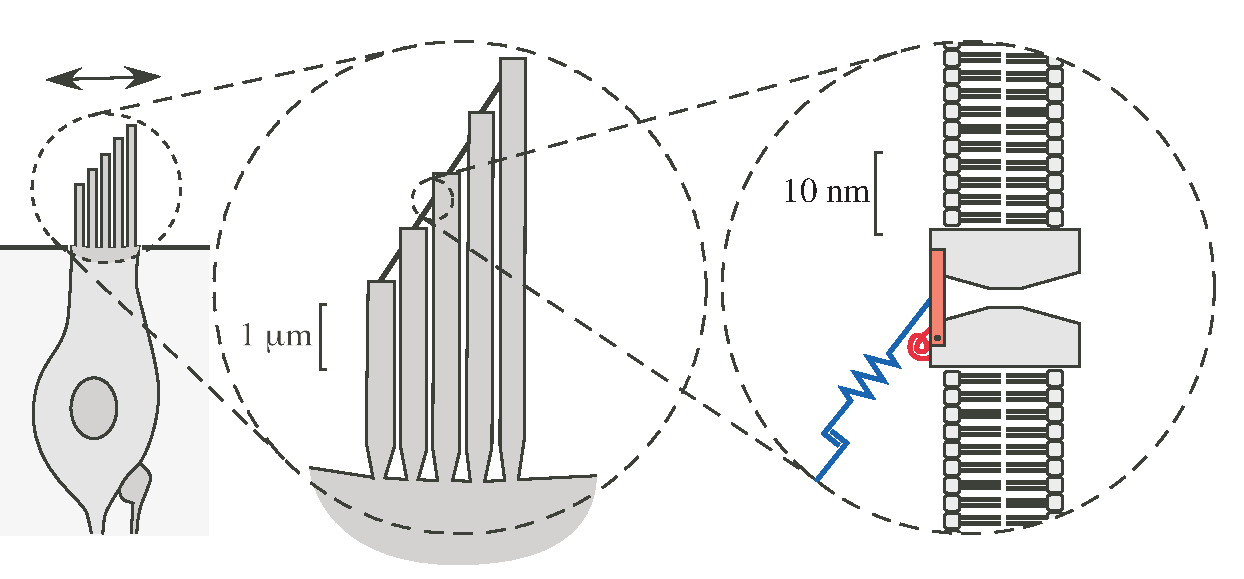
\includegraphics[width=0.8\linewidth]{ExampleFigure} % For Mac OS X PDFs (else append .eps)
		\caption{Figure captions go on bottom.}
		\label{SchematicDiagram}
	\end{center}
\end{figure}

Finally, we can also include tables, such as Table \ref{demoTable}. Like figures, we can also \emph{attempt} to force their positions. 

In the document class line, we can easily convert from ``preprint" one-column, double-spacing for rough drafts to ``twocolumn" single spacing for final drafts! 

This is dummy text. This is dummy text. This is dummy text. This is dummy text. This is dummy text. This is dummy text. This is dummy text. This is dummy text. This is dummy text. This is dummy text. This is dummy text. This is dummy text. This is dummy text. This is dummy text. This is dummy text. This is dummy text. This is dummy text. This is dummy text. This is dummy text. This is dummy text. This is dummy text. This is dummy text. This is dummy text. This is dummy text. This is dummy text. This is dummy text. 

\begin{table}[h] % indenting is optional	
	\caption{Table captions go on top.}
	\label{demoTable}
	\begin{center}
		\begin{tabular}{cc} % "cc" = center each column
			absicssa & ordinate\\
			\hline
			1.0 s & 5.6 m\\
			2.0 s & 6.7 m\\
			3.0 s & 9.9 m
		\end{tabular}
	\end{center}
\end{table}

%%%%%%%%%%%%%%%%%%%%%%%%%%%%%%%%%%%%%%%%
%%%%%%%%%%%%%%%%%%%%%%%%%%%%%%%%%%%%%%%%
\chapter{Conclusions}\label{Conclusions}

\section{Stuff}
This is dummy text. This is dummy text. This is dummy text. This is dummy text. This is dummy text. This is dummy text. This is dummy text. This is dummy text. This is dummy text. This is dummy text. This is dummy text. This is dummy text. This is dummy text. This is dummy text. This is dummy text. This is dummy text. This is dummy text. This is dummy text. This is dummy text. This is dummy text. This is dummy text. This is dummy text. This is dummy text. This is dummy text. This is dummy text. This is dummy text. 

This is dummy text. This is dummy text. This is dummy text. This is dummy text. This is dummy text. This is dummy text. This is dummy text. This is dummy text. This is dummy text. This is dummy text. This is dummy text. This is dummy text. This is dummy text. This is dummy text. This is dummy text. This is dummy text. This is dummy text. This is dummy text. This is dummy text. This is dummy text. This is dummy text. This is dummy text. This is dummy text. This is dummy text. This is dummy text. This is dummy text. 


%%%%%%%%%%%%%%%%%%%%%%%%%%%%%%%%%%%%%%%%
%%%%%%%%%%%%%%%%%%%%%%%%%%%%%%%%%%%%%%%%
\appendix

\noappendicestocpagenum	 % suppress page number ...
\addappheadtotoc	% ... but add appendices header to table of contents 

\renewcommand{\theequation}{A-\arabic{equation}} % redefine the command that creates the equation number
\setcounter{equation}{0}  % reset counter 

\renewcommand{\thesection}{A-\arabic{section}} % redefine the command that creates the section number
\setcounter{section}{0}  % reset counter 

\renewcommand{\thetable}{A-\arabic{table}} % redefine the command that creates the table number
\setcounter{table}{0}  % reset counter 

%%%%%%%%%%%%%%%%%%%%%%%%%%%%%%%%%%%%%%%%
%%%%%%%%%%%%%%%%%%%%%%%%%%%%%%%%%%%%%%%%
\chapter{Extra Stuff}\label{Extra}

This is dummy text. This is dummy text. This is dummy text. This is dummy text. This is dummy text. This is dummy text. This is dummy text. This is dummy text. This is dummy text. This is dummy text. This is dummy text. This is dummy text. This is dummy text. This is dummy text. This is dummy text. This is dummy text. This is dummy text. This is dummy text. This is dummy text. This is dummy text. This is dummy text. This is dummy text. This is dummy text. This is dummy text. This is dummy text. This is dummy text. 

This is dummy text. This is dummy text. This is dummy text. This is dummy text. This is dummy text. This is dummy text. This is dummy text. This is dummy text. This is dummy text. This is dummy text. This is dummy text. This is dummy text. This is dummy text. This is dummy text. This is dummy text. This is dummy text. This is dummy text. This is dummy text. This is dummy text. This is dummy text. This is dummy text. This is dummy text. This is dummy text. This is dummy text. This is dummy text. This is dummy text. elegant text. This elegant text. This elegant text. This elegant text. This elegant text. 

%%%%%%%%%%%%%%%%%%%%%%%%%%%%%%%%%%%%%%%%
%%%%%% *-%%%%%%%%%%%%%%%%%%%%%%%%%%%%%%%%%
\chapter{Extra Stuffing}\label{Stuffing}
This is dummy text. This is dummy text. This is dummy text. This is dummy text. This is dummy text. This is dummy text. This is dummy text. This is dummy text. This is dummy text. This is dummy text. This is dummy text. This is dummy text. This is dummy text. This is dummy text. This is dummy text. This is dummy text. This is dummy text. This is dummy text. This is dummy text. This is dummy text. This is dummy text. This is dummy text. This is dummy text. This is dummy text. This is dummy text. This is dummy text. 

This is dummy text. This is dummy text. This is dummy text. This is dummy text. This is dummy text. This is dummy text. This is dummy text. This is dummy text. This is dummy text. This is dummy text. This is dummy text. This is dummy text. This is dummy text. This is dummy text. This is dummy text. This is dummy text. This is dummy text. This is dummy text. This is dummy text. This is dummy text. This is dummy text. This is dummy text. This is dummy text. This is dummy text. This is dummy text. This is dummy text. 

%%%%%%%%%%%%%%%%%%%%%%%%%%%%%%%%%%%%%%%%
%%%%%%%%%%%%%%%%%%%%%%%%%%%%%%%%%%%%%%%%
%%%%%%%%%%%%%%%%%%%%%%%%%%%%%%%%%%%%%%%%
\backmatter

\addcontentsline{toc}{chapter}{Bibliography}
\bibliography{thesis}
%\bibliographystyle{plain}			% listed alphabetically but ordered numerically, including titles
\bibliographystyle{unsrt}			% like plain but references appear in order of citation
%\bibliographystyle{alpha}		% like plain, except reference labels used
%\bibliographystyle{abbrv}		% like plain, but abbreviations uses for authors first names, etc.

\end{document}